%File: MUME_paper.tex
\documentclass[letterpaper]{article}
\usepackage{MUME}
\usepackage{graphicx}
\usepackage{caption}
\usepackage{subcaption}
\usepackage{amsmath}
\usepackage{times}
\usepackage{helvet}
\usepackage{courier}
\usepackage{url}

\newcommand\mydots{\hbox to .75em{.\hss.\hss.}}
\frenchspacing
\setlength{\pdfpagewidth}{8.5in}
\setlength{\pdfpageheight}{11in}

\graphicspath{ {images/} }

\pdfinfo{
/Title (HBPL: a Framework for Debating, Developing, and Reusing Foundational Models of Musical Metacreativity)
/Author (Paul Bodily, Dan Ventura)}
\setcounter{secnumdepth}{0}  
\begin{document}
% The file MUME.sty is the style file for MUME 
% proceedings, working notes, and technical reports.
% \author{Paul Bodily, and Dan Ventura\\

\title{HBPL: a Framework for Debating, Developing, and\\Reusing Foundational Models of Musical Metacreativity}
\author{Paul Bodily and Dan Ventura\\
Computer Science Department\\
Brigham Young University\\
Provo, UT 84602  USA\\
paulmbodily@gmail.com, ventura@cs.byu.edu\\
}
\maketitle
\begin{abstract}
\begin{quote}
A modular framework for musical metacreativity (MUME) promotes several desirable attributes of MUME systems, namely opportunities for model reuse, collaboration, and focused debate on subproblem solutions. We argue that hierarchical Bayesian program learning (HBPL) is an ideal framework for MUME systems because of its ability to effectively learn by modularly decomposing concepts into independently-learned subconcept models. We illustrate how the framework can be used to model music composition. Because subconcept models represent musical constructs, the language of the framework can be used for articulating and comparing different perspectives of the music composition process. We use the framework to examine differing perspectives on the relationships between the concepts of harmony and melody and between melody and lyrics.
\end{quote}
\end{abstract}

\section{Introduction}

Many aspects of music are modular and there is significant commonality in the subsystems required for implementing musical metacreativity (MUME) systems across genres or problem domains. Although new systems in MUME often reuse and develop upon ideas or ``approaches'' presented in previous systems, the reuse of specific subsystem models (trained or untrained) is rare. For example, models of harmonic progression are frequently used in systems ranging from classical to jazz to pop music, however even systems within these domains (let alone between them) reimplement these models time and again. Of course model parameters may be different for each domain, but a general concept of what harmony \emph{is} and how it relates to composition is at some level the same across domains. The dominant-tonic cadence, for example, may occur with different frequencies or in different places in jazz than it does in classical; however the definitions of dominant, tonic, and a dominant-tonic cadence largely remain the same. It is important to clarify that independent of \emph{which} models are reusable across systems, at least \emph{some} such models do exist. Having models that can be reused, potentially with a set of possible domain-specific parameterizations would be a valuable resource for the MUME research community at large.

MUME systems stand to benefit from code and model reuse for multiple reasons. Most obviously there are significant time and energy savings to reusing existing models. Perhaps most significant, however, is that through their reuse such models undergo iterative improvements, resulting in refined models that lay a foundation for being able to do more effective research using these models.

Given the apparent advantages to model reuse, why is it not more widely observed? We first discuss two ideas challenges to model reuse. We then devote the remainder of the paper to presenting a framework that addresses these challenges. We demonstrate how having such a framework facilitates meaningful discussion and reuse of submodels of musical metacreativity. 

\subsection{Modularization}

Modularizing systems encourages both reusing modules developed for the modularized system \emph{and} reusing the system with replacement of specific modules. For example, a MUME system may have a very powerful model for generating melody. Modularizing the system so that the melody model can be easily repurposed encourages its reuse. Alternatively, a MUME system may have a weak model for generating melody, but is otherwise a very effective system. Modularizing the system so that an alternative melody model can be either developed \emph{de novo} or reused from another existing system also encourages reuse. In both cases, modularization allows the best of multiple systems to be recombined to create potentially better systems of musical metacreativity.

A challenge, however, is deciding how and at what level modularization should take place. At the highest level of modularization, a complete MUME system has limited reusability. For example, there are a limited number of novel systems that can be developed from reusing a system like SMUG \cite{scirea2015smug} that generates lyrical music inspired by academic papers. However, the lower-lever submodel used \emph{within} SMUG to generate melody (as a combination of pitch and rhythm), is likely reusable in developing novel systems.

Focusing on lower level modules has two distinct benefits: first, lower level modules affect MUME systems across a greater breadth of sub-domains; and second, lower level modules represent an important foundation for building effective higher-level modules (see Figure~\ref{fig:modularization_levels}). Focusing on these lower level models provides a way for the MUME community to share knowledge and build fundamental models of music that can then be used to improve domain-specific systems. 

\begin{figure}
	\centering
	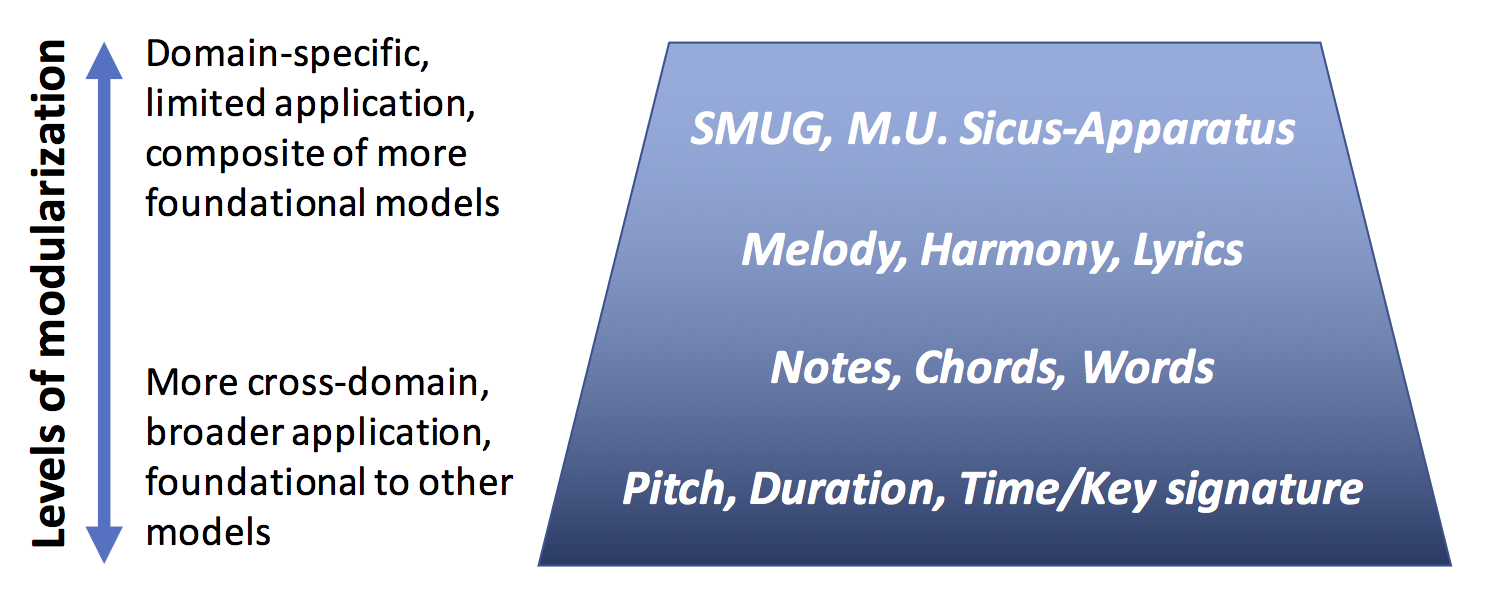
\includegraphics[width=\linewidth]{modularization_levels_gradient}
	\caption{\label{fig:modularization_levels} The pyramid shows examples of concepts at different levels of modularization. The highest level modules represent full-functioning MUME systems (e.g., SMUG \cite{scirea2015smug} and M.U. Sicus-Apparatus \cite{toivanen2013automatical}) which are composed of lower level modules and have more narrow applications. Lower level modules represent subconcepts that are more broadly applicable and are foundational to more complex concepts. A modular approach to building MUME systems focuses on developing (potentially reusable) models at multiple levels.}
\end{figure}

Often it may seem that different musical viewpoints (e.g., pitch, rhythm) are too interdependent to allow effective modularization of a system. While this certainly poses a challenge, models need not be independent in order to be modularized. For example, a model of melody conditioned on harmony is very valuable even without a model of harmony.

\subsection{Lingua Franca}

Some existing MUME systems which \emph{do} take modular approaches discourage reuse due to communication barriers. Effective reuse requires knowing when and how a model can be reused. While precision is important for evaluating the suitability of a model for reuse, extensive mathematical formulations sometimes deter system designers from investing the time required to learn how and if to use prebuilt models. On the other hand, some models are described in insufficient detail, making it impossible to determine what assumptions the model makes or how it is to be used.

Beyond failing to understand a specific model, there is a general need for a language, a framework, and a culture that encourages and facilitates model reuse. While we share the language of music and the language of computational science, neither language represents a framework for discussing the higher-order elements of composition/song-writing. As such, many new systems inadvertently create novel frameworks in addition to presenting new ideas. This lack of a consistent framework can make it difficult to identify and interpret reusable models. More generally, this lack of a common language limits our ability to join in constructive, communal discussion, making it difficult to engage in a persistent dialog about the relative effectiveness of different (reusable) models or how models can be most effectively combined in new systems.

\section{Hierarchical Bayesian Program Learning}

The purpose of this paper is to propose a framework that addresses these challenges and initiate a discussion about some aspects of MUME using the framework. The framework we are proposing is the hierarchical Bayesian program learning (HBPL) framework \cite{lake2015human}. As applied to music, HBPL describes a hierarchy of probabilistic models that are designed to learn the subconcepts that make up musical composition. By empirically learning subconcepts, the aggregate model is then able to comprehend examples of composition beyond those seen in training.

The framework's potential for learning complex concepts was recently demonstrated on hand-written characters. In \citeauthor{lake2015human}'s model, a character type $\psi$ is learned as a product of learning distributions for the number of strokes $\kappa$ per character, the number of substrokes $n_i$ per stroke, the substroke shape $S_i$, and the relationship $R_i$ between strokes:
\[ P(\psi) = P(\kappa) \prod_{i=1}^{\kappa} P(n_i|\kappa)P(S_i|i,n_i)P(R_i|S_1, ..., S_{i-1}). \]

As demonstrated in this example, an HBPL model defines a joint distribution over some class of artefact as a factorization into probabilistic distributions representing subconcepts. By learning each of these subconcepts individually, the model was shown to achieve human-level concept learning in tasks such as one-shot classification, parsing, and generation.

\section{Defining A Composition}

By its nature the HBPL model necessitates defining the concepts to be modeled in terms of constituent subconcepts. Because this essentially represents manually incorporating high-level knowledge about music composition into the system, this process of defining can be both a strength and a weakness. If done effectively it results in a very powerful model (as demonstrated by \citeauthor{lake2015human} \shortcite{lake2015human}). If done poorly it limits the learning ability of the system. Although there are likely few who would contest the manner in which \citeauthor{lake2015human} defined hand-written characters, there is likely to be more disagreement about how music composition should be defined. One advantage to the HBPL framework is the opportunity to engage MUME researchers and musicians alike in this debate, not simply to converge on a single definition, but to examine and compare several.

At the highest level we must define the concept of music composition itself.  It is significant to note that the model of character types presented by \citeauthor{lake2015human} was designed to learn characters generally and not to cater to any specific language or context (though it was shown to be capable of modeling different alphabets). By analogy whatever our definition for composition\footnote{By \emph{composition} we refer to the \emph{symbolic} representation of a musical piece} it must be comprehensive enough to include jazz, classical, pop, handbell choir, a cappella, and any other type of music composition. Our definition should be such that the difference in composition between domains can be expressed as a function of the submodel parameters.

A composition is typically defined in terms of \emph{viewpoints}. For example, \citeauthor{conklin1995multiple} define a chorale as a ``discrete event sequence'' with each event representing the viewpoints of pitch, key signature, time signature, fermata, start time, and duration \shortcite{conklin1995multiple}. \citeauthor{pachet2014imitative} define a jazz leadsheet as consisting of ``two `parallel' sequences: one that contains chord labels and one that contains notes'' \shortcite{pachet2014imitative}. \citeauthor{bodily2017ICCC} similarly define a lyrical composition as consisting of \emph{three} parallel sequences: one for chord labels, one for notes, and one for lyrics \shortcite{bodily2017ICCC}. \citeauthor{cope1989experiments}'s EMI is a notable example of a non-linear model of composition, but which nonetheless focuses on the recombination of patterns in the viewpoints of pitch and duration \shortcite{cope1989experiments}.

These examples suffice to demonstrate that although a composition is often defined using multiple viewpoints, models vary widely as to the specific viewpoints they consider. We thus define a \emph{universal distribution over compositions} $\gamma$ as
\[ P(\gamma) = P(V_1) P(V_2|V_1), \mydots, P(V_n|V_1,\mydots,V_{n-1}) \]
\noindent where $U = (V_1, \mydots, V_n)$ represents the set of all possible viewpoints that can be defined for a composition. Put simply: a composition is a factorable distribution over viewpoints. Given this definition, we make a few important observations.

First, by Bayes' Law the exact ordering of dependencies between viewpoints is (at least in theory) unimportant to modeling $P(\gamma)$. For example, for a composition $\gamma'$ which defines two viewpoints, $V_1$ and $V_2$:
\[ P(\gamma') = P(V_1) P(V_2|V_1) = P(V_2) P(V_1|V_2). \]

The point to be made here is that to the extent that subconcept models are accurate, the exact factorization of $P(\gamma')$ is irrelevant. In practice we make independence assumptions in an effort to compensate for data sparsity. This results in only approximative subconcept models with the choice of factorization resulting in different approximations of the joint distribution. Thus how we factor becomes an important part of the discussion of how hierarchical models should be structured.

\begin{figure}[th]
    \centering
    \begin{subfigure}[b]{.5\textwidth}
        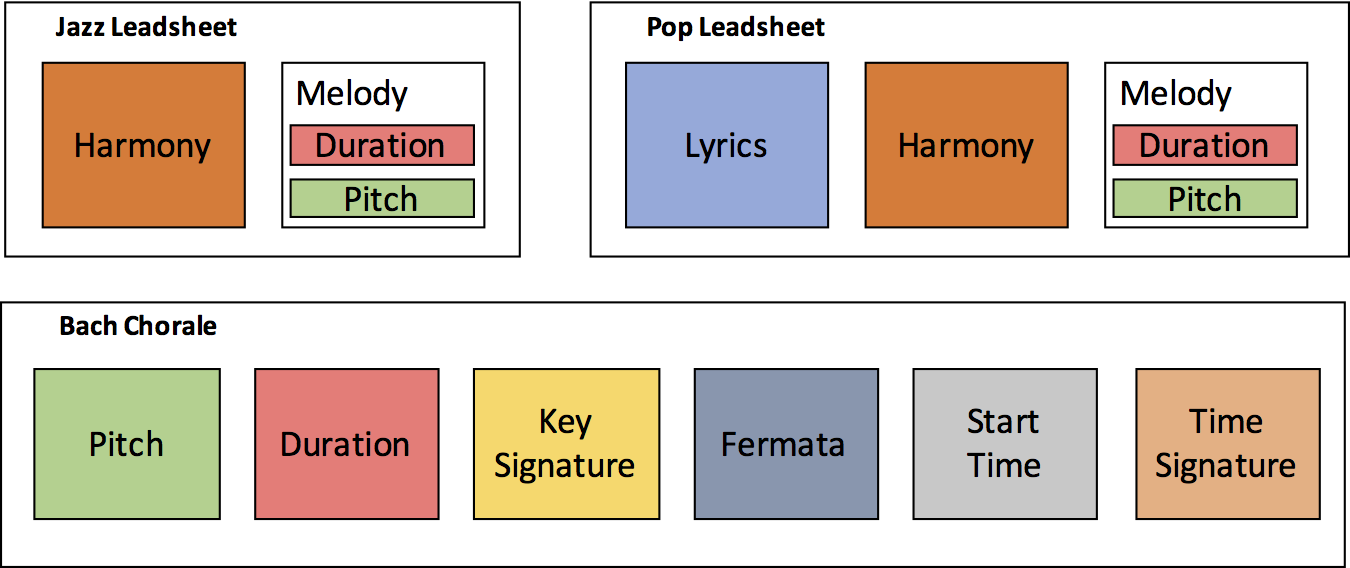
\includegraphics[width=\textwidth]{unoverlapping_models}
        \caption{Modular systems without reuse}
        \label{fig:unoverlapping}
    \end{subfigure}
    \\~\\ %add desired spacing between images, e. g. ~, \quad, \qquad, \hfill etc. 
    %(or a blank line to force the subfigure onto a new line)
    \begin{subfigure}[b]{.5\textwidth}
        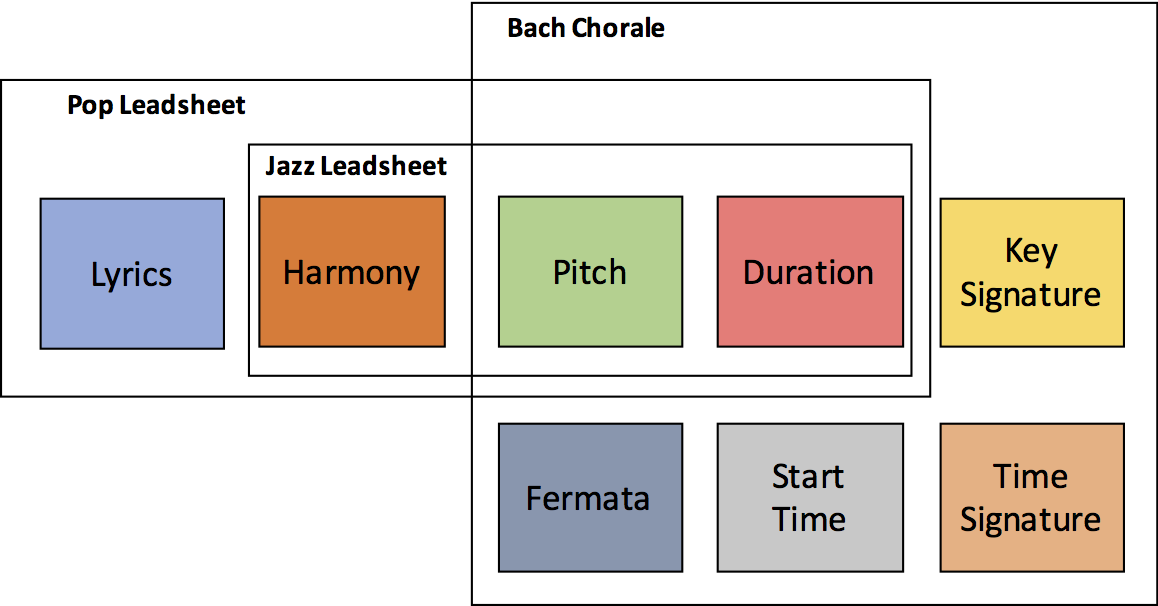
\includegraphics[width=\textwidth]{overlapping_models}
        \caption{Modular systems with reuse}
        \label{fig:overlapping}
    \end{subfigure}
    \caption{\emph{Modularizing with reuse}. (a) Three different models of composition defined according to their constituent subconcept models (each unique subconcept has a unique color). (b) The same three models of composition defined using common subconcept models. This overlap suggests opportunities for reuse and collaboration.}\label{fig:modularization}
\end{figure}

Second, different types of composition which recognize a subset of viewpoints $S \subset U$ can be derived from compositions which recognize a larger subset of viewpoints $S'$ (s.t. $S \subset S' \subseteq U$) by marginalizing over variables $V_i \in S'-S$. For example, a specialized composition $\gamma'$ which defines all viewpoints $V_i \in U$ except the viewpoint $V_1$ is derived from the universal distribution $P(\gamma)$ as follows:
\begin{align*}
P(\gamma') &= \int_{V_1} P(\gamma) dV_1\\ 
&= \int_{V_1} P(V_1) P(V_2|V_1), \mydots, P(V_n|V_1,\mydots,V_{n-1}) dV_1\\ 
&= P(V_2), \mydots, P(V_n|V_2,\mydots,V_{n-1})
\end{align*}

As a more concrete example, consider that a definition of jazz leadsheets which defines viewpoints of harmony, duration, and pitch can be derived from a definition of pop leadsheets which defines viewpoints of harmony, duration, pitch, and lyrics by marginalizing over lyrics. In simple terms, an effective model built for pop leadsheets could be repurposed to build jazz leadsheets by ignoring lyrics and retraining parameters for jazz composition. In general this suggests that there are often ways of converting existing models from one to another through conditioning and marginalizing over variables. This observation is valuable because it suggests there are likely many ways in which existing models can be modularized to allow their submodels to be reused for novel systems or purposes (see Figure~\ref{fig:modularization}).

Third, note that there is also another implication for reusable models: two specialized compositions $\gamma'$ and $\gamma''$, despite marginalizing over subsets $S'$ and $S''$ s.t. neither is a strict subset of the other, may have overlapping factors so that a conditional model for the viewpoint $V_i$ in the factorization of $\gamma'$ is similarly required and conditioned in $\gamma''$. Consider that \citeauthor{conklin1995multiple}'s model of Bach chorales includes models of pitch and duration that could be reused as a submodel for modeling lyrical composition or jazz composition (see Figure~\ref{fig:modularization}).

We reemphasize that we are \emph{not} suggesting that the \emph{trained} pitch model of \citeauthor{conklin1995multiple} built for Bach chorales can be reused \emph{as is} in a system that models pop or jazz leadsheet composition. It is probable that some \emph{retraining} of parameters on data more representative of the subdomain will be necessary. But the \emph{definition} of the pitch model \emph{can} be reused between different domains. As a very simple example, consider a model of pitch that is approximated using a single-order Markov model. This clearly represents a model of pitch that could be (and has been) reused (with different parameters) in several subdomains. So likewise one might imagine more complex approximative models being reusable to represent common subconcepts.

There exists some tendency on the part of individuals in both in the world of music and in the world of musical metacreativity to elevate some types of music as being intrinsically more sophisticated or valuable and to ignore any but those models and contributions belonging to one's own subdomain of interest. While each is entitled to his or her own opinion, the ability to reach beyond differences and identify what these domains have in common holds the promise to more efficiently achieving our mutual goals. Musical metacreativity relies on the ability of systems to firmly grasp very simple concepts in music, concepts which are often not domain-specific, concepts which though simple need to be modeled and evaluated thoroughly. There is a great opportunity for musical metacreativity designers to collaborate in modeling fundamental aspects of music that can then be used as a common knowledge base from which to build more complex, domain-specific systems. 

As has been demonstrated, the challenges posed by implementing systems using an HBPL model in actuality represent very concrete opportunities for debate, discussion, and research about
\begin{enumerate}
\item how to identify and define simple, reusable musical concept models;
\item how to create more complex concept models from simpler subconcept models;
\item how well different implementations serve to approximate a specific subconcept; and
\item how to encourage and classify contributions to MUME research along a spectrum of domain-specificity ranging from fundamental submodels of general music concepts to more aggregate models of (potentially genre-specific) musical concepts.
\end{enumerate}
\noindent In short, such a framework helps orchestrate a combined effort to discover subconcepts in music whose definition we \emph{can} usefully agree upon. Initially these are likely to be fairly fundamental subconcepts, whose definition may then facilitate defining more aggregate concepts.

\section{Model of Lyrical Composition}

To demonstrate the process of defining a specific type of composition using the HBPL framework, we consider the problem of modeling lyrical composition.

\begin{figure*}[th]
	\centering
	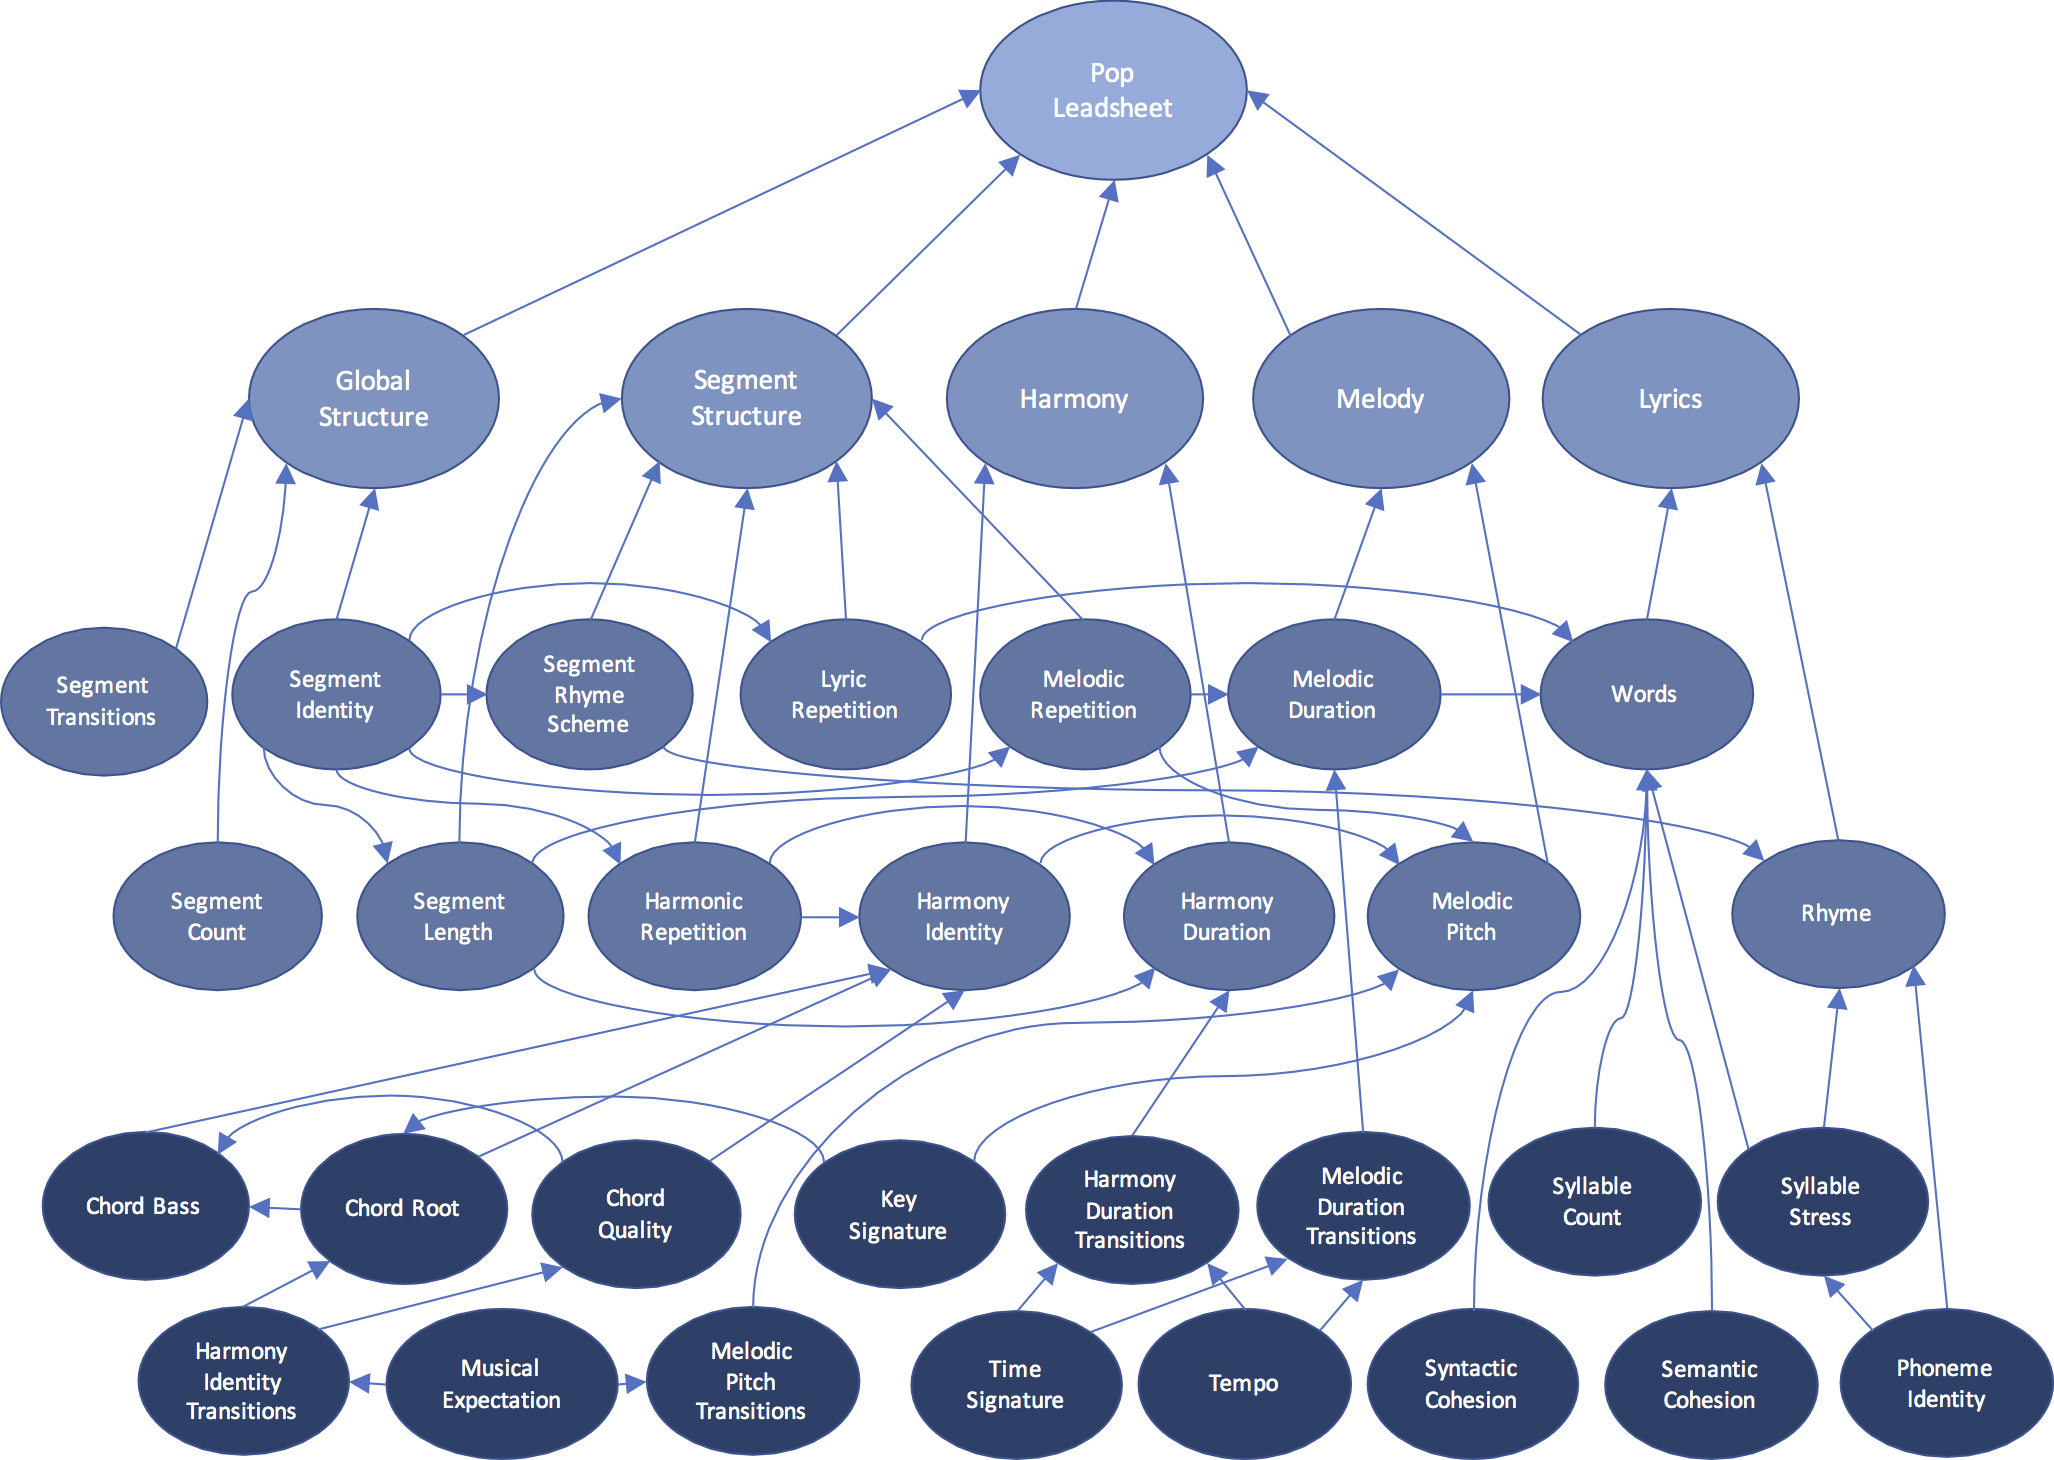
\includegraphics[width=\linewidth]{pop_hbpl_gradient}
	\caption{\label{fig:pop_hbpl_gradient} A graphical model of one possible hierarchy for defining a pop leadsheet using the HBPL framework. Each node represents a concept or subconcept model used to define pop leadsheet composition. The vertical layers in the graph correspond roughly to the levels of modularization shown in Figure~\ref{fig:modularization_levels}. An arrow from a node $A$ to a node $B$ represents that $B$ is conditioned on $A$. As is needed for an HBPL model, no circular dependencies exist. The model is sampled from the bottom up.}
\end{figure*}

Figure~\ref{fig:pop_hbpl_gradient} shows one possible hierarchy for defining a pop leadsheet using the HBPL framework. There are several things to note about this figure. The graph represents valuable domain-specific knowledge. Although some of the concepts and dependencies (shown as arrows) may be debated, such a hierarchical model provides an excellent starting point for talking about what a concept graph of pop leadsheet composition \emph{should} look like, and we hypothesize that some evolution of this graph is likely to be very effective at producing pop music. Many of these are concepts that are very intuitive and are modeled in many different MUME systems. Note that the bottom layer represents primarily concepts that are fundamental to many genres of music and/or literature. Defining a pop leadsheet in this manner also helps to initiate a discussion and comparative analysis of possible implementations for approximating each individual subconcept. 

We now explore a few examples of the type of discussions that we hope to see emerge from models like that shown in Figure~\ref{fig:pop_hbpl_gradient}. We discuss the motivation for including the concepts of \emph{Global Structure} and \emph{Segment Structure}. We then discuss the intuition behind two dependence relationships in this graph that were significantly debated in the construction of this model.

For the purposes of our discussion, we define a simplified HBPL model of the conditional distribution on compositions $\gamma$ as follows
\begin{equation}
P(\gamma) = P(\tau)P(\eta|\tau)P(\mu|\tau,\eta)P(\lambda|\tau,\mu) \label{eq}
\end{equation}
\noindent where the variables $\tau$, $\eta$, $\mu$, and $\lambda$ respectively represent the composition's structure (global and segment-level), harmony, melody, and lyrics\footnote{An implementation of this model is described in \cite{bodily2017ICCC}. Compositions generated from this implementation are available online at \url{popstar.cs.byu.edu}}.

\subsection{Structure}

Though not representative of \emph{concrete} viewpoints of composition, structure (e.g., verse-chorus segmentation, rhyme scheme, etc.) is a concept so frequently discussed in association with pop leadsheets that it becomes inconvenient \emph{not} to explicitly model it. This represents an additional strength of the HBPL model, namely that composition can be explicitly modeled in terms of any relevant concept, including concepts such as inspiration and intention \cite{bodily2017ICCC}. 

Several attempts have been made to learn to generate music \emph{without} explicitly modeling structure (e.g., \cite{van2016wavenet}). Although these systems are often able to generate small windows of realistic sounding music, on the whole they lack the structure needed to create broader cohesion.

We further decompose our model of structure as
\[ P(\tau) = P(\zeta)P(\sigma|\zeta), \]
\noindent where \(P(\zeta)=\) distribution over global structure $\zeta$ and \(P(\sigma|\zeta)=\) distribution over segment structure $\sigma$ given $\zeta$.

\subsubsection{Global Structure}
The dividing of the composition into verse-chorus segments is represented in Figure~\ref{fig:pop_hbpl_gradient} as \emph{Global Structure}. As an example of how we might implement a subconcept model, one way of modeling global structure is to use a \textit{constrained Markov model}. According to this model $P(\zeta)$ is factored into a distribution over the segment count per song, $P(|\zeta|)$, and a single-order Markov model for segment sequences:
\[ P(\zeta) = P(|\zeta|) P(\zeta_1) \prod_{i=2}^{|\zeta|} P(\zeta_i|\zeta_{i-1}). \]

Using an unconstrained, unsmoothed Markov model for $P(\zeta_i|\zeta_{i-1})$ may result in sequences shorter than $|\zeta|$ and may end unnaturally (e.g., with a bridge). Using \citeauthor{pachet2001finite}'s \emph{constrained} Markov model we can guarantee the sequence length and place additional constraints at specific positions within the sequence. This modifies how we factor $P(\zeta)$ by conditioning $\zeta_i$ on both the sequence position $i$ and the previous segment type $\zeta_{i-1}$:
\[ P(\zeta) = P(|\zeta|) P(\zeta_1) \prod_{i=2}^{|\zeta|} P(\zeta_i|i,\zeta_{i-1}) \]
To generate, we sample a length from $P(|\zeta|)$ and construct a constrained Markov model of length $|\zeta|$ using $P(\zeta_i|\zeta_{i-1})$. We also add a constraint that the song must end on an ``end'' token. 

This model does well at creating compositions that have a reasonable number of verse-chorus segments and that start and end appropriately. However, with only a single-order Markov model underlying the constrained model, there is likely to be some odd placement of segments \emph{within} the structure. For example, training data may contain examples of a bridge following a chorus, but not generally the \emph{first} chorus. A single-order Markov model would have insufficient context to discriminate between chorus instances. Thus it might be better to try a higher-order constrained Markov model, some sort of generative grammar (e.g., \cite{steedman1984generative}), or even some sort of recurrent neural network. These are all likely to produce better global structures than the model shown here.

This example serves to demonstrate how the modularity of the HBPL framework facilitates focused comparative analysis across implementations for a given subconcept model.

\subsubsection{Segment Structure}

As referred to in Figure~\ref{fig:pop_hbpl_gradient}, \emph{Segment Structure} refers to lyrical, melodic, or harmonic motifs and rhyme schemes within a segment (e.g., verse).  This structure can be essentially defined as a set of constraints $C_i$ on various viewpoints of the composition at certain measure and beat positions \cite{bodily2017ICCC}. Many systems that use constraints require the user to define the constraints (e.g., \cite{pachet2014imitative}). Using the HBPL framework, we can create a model to learn the concept of how constraints are defined. Figure~\ref{fig:segment_structure} shows an example of an empirically derived probability distribution over rhyme constraints that might be used to approximate a subconcept model of segment structure.

\begin{figure}
	\centering
	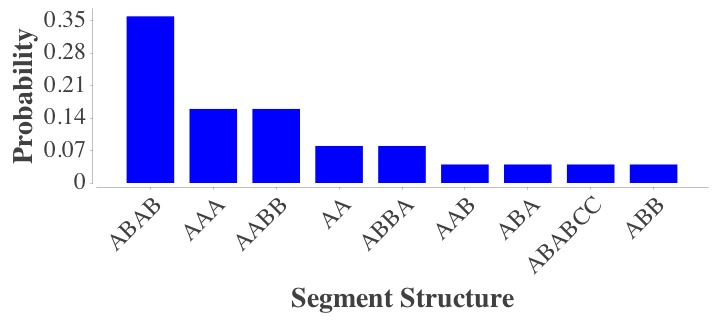
\includegraphics[width=\linewidth]{segment_structure}
	\caption{\label{fig:segment_structure} A visual representation of an empirically derived probability distribution for a subconcept model of song segment rhyme structure.}
\end{figure}

The major qualm we have with this model is that motifs not only exist \emph{within} segments, but also \emph{between} segments. Our current model samples a new $C_i$ for each segment type independently of all other segment types. For example, chord patterns often repeat in the intro, outro, chorus, and verse in ways that create global cohesion to the composition. A better model might condition the segment structure of one segment on the structures of previous segments.

In general, modeling structure has proven to be one of the more challenging and most interesting concepts to define. We hope to leverage community discussion and domain knowledge to improve our models of global and segment structure for future work.

\subsection{Harmony and Melody}

Figure~\ref{fig:pop_hbpl_gradient} shows that the model of \emph{Melodic Pitch} depends on (among other concepts) \emph{Harmony Identity}. This represents the assertion (also reflected in Equation~\ref{eq}) that melody is determined from harmony. Among those of our colleagues who first reviewed this model, many asserted that this was a backward assumption and that harmony is actually derived from the melody. Presumably this notion was driven by the prominent role that melody plays in identifying a composition. Systems have also been designed which generate harmony from melody \cite{chuan2011generating}.Thus we find it meaningful to provide some defense for our assertion.

As noted above, whether melody $\mu$ is conditioned on harmony $\eta$ or harmony on melody is in theory irrelevant:
\begin{align*}
P(\mu, \eta) &= P(\mu) P(\eta|\mu) \\
&= P(\eta) P(\mu|\eta);
\end{align*}
\noindent the same model of harmonized melody is computable either way. However, as also noted above, practice does not always agree with theory. Consider if, in implementing melody, we (na\"{i}vely) choose to use a 0-order Markov model such that each note is sampled independent of the previous note. Conditioning $\eta$ on $\mu$ in this manner would be akin to playing random notes in sequence and then trying to determine a chord from those notes. Conditioning $\mu$ on $\eta$ would be akin to choosing a chord and then playing random notes from the chord. Though neither is likely to produce a well-shaped melody, the latter seems more likely to evoke a stronger sense of musical cohesiveness.

Others have also supported this assertion. For example, \citeauthor{papadopoulos1999ai} assert that melody does not stand alone and must be evaluated according to the ``harmonic context'' \shortcite{papadopoulos1999ai}. This assumption also follows from the definition of tonality, which designates that pitch is arranged around a contextual reference point \cite{hyer2001}. \citeauthor{paiement2005chord} note that harmony \emph{is} dependent on ``chord structure... and on the surrounding chords,'' but make no mention of its dependence on melody \shortcite{paiement2005chord}. \citeauthor{dixon2010probabilistic} also state that ``since the highest number of dependencies join at the chord variable, it takes a central position in the network'' \shortcite{dixon2010probabilistic}.

This example demonstrates a few things. First, it demonstrates HBPL models can be built which reflect the knowledge of domain experts. Second, it demonstrates that a dialogue among these experts is important to being able to discover how such models should be effectively constructed.

\subsection{Melody and Lyrics}

Figure~\ref{fig:pop_hbpl_gradient} shows that the model of \emph{Words} depends on (among other concepts) \emph{Melodic Duration}. This represents the assertion (also reflected in Equation~\ref{eq}) that lyrics are determined from melody. This assertion is one that we have internally debated for some time due to the complexity of the interaction between these two viewpoints.

It is clear that there is some dependency between melody and lyrics: in pop music, syllables usually correspond to notes in the melody and vice versa. \emph{How} melody and lyrics depend on each other is more complex, particularly given that MUME systems exist which create lyrics for melodies \cite{ramakrishnan2009automatic} and melodies for lyrics \cite{monteith2012automatic}. This complexity may be what drives the common question posed to song-writers: ``which do you write first: the melody or the lyrics?'' Consider that the question is meant to gauge individual styles of song-writing rather than inquiring as to whether or not the song-writer adheres to a universally agreed upon principle of song-writing. This means that different people successfully write music in different ways. Answers vary from ``always melody first'' to ``always lyrics first'' to ``they come at the same time'' to ``it varies'', but each answer reflects an effective model of how songs are written. 

The fact that those who ask this question appreciate music either way suggests that the order in which one writes the melody and lyrics of a song is perhaps not important. Furthermore, the fact that those who ask this question rarely try to guess the answer suggests that the order in which one writes the melody and lyrics of a song is not readily reflected in the resulting composition. (Beyond its implications for how to design a generative model, this represents an interesting method for evaluating the effectiveness of an HPBL model: a model is likely to be a more effective model if, like human-written songs, listeners cannot accurately determine the order in which lyrics and melody are generated.)

The HPBL framework is capable of modeling a system that generates lyrics and melody in either order, but we have found that when it comes to implementation there are a few factors to be considered.

First, the general \emph{contour} of the melody (e.g., ``PACTs'' as presented by \citeauthor{pachet1991representing} \shortcite{pachet1991representing}) \emph{is} independent of the lyrics as evidenced by the fact that such contour is consistent across several verses with different lyrics (this is not to say that the contour is not somehow dependent on the overall semantic meaning of the song). This is the intuition reflected in our assertion that the lyrics depend on the melody and not the other way around.

However, the second factor to consider is that there are multiple elements of melody that \emph{do} depend on the lyrics. This is essentially what is meant by the term \emph{prosody}. Although the \emph{contour} of the melody may be independent of the verse lyrics, the \emph{rhythm} of the melody certainly depends on the lyrics: the number of notes and syllables must agree and the exact rhythm of notes is (at least in part) a function of the stress patterns in the lyrics. Even the pitch of the melody is occasionally modified to accentuate the semantic meaning of the associated lyrics.

This example demonstrates that we must think carefully about how we define the concepts that are used to define an HBPL model. Some of these concepts (like prosody) are powerful concepts for evoking the perception of creativity, but are not often incorporated into MUME systems because of the time required to (re)implement more fundamental concepts like harmony, melody, and lyrics. Establishing a common framework like HBPL, by which to share not just ideas but actual models of musical concepts, enables researchers to focus efforts on how to combine and reuse existing models, allowing more time to be devoted to incorporating other less-common, essential concept models. \emph{Musical Expectation} (shown in Figure~\ref{fig:pop_hbpl_gradient}) is another example of a powerful concept that we feel should see more wide use in MUME systems \cite{meyer2008emotion}.

\subsection{HBPL: Reaching the boundary of Creativity}

Let us return for a moment to the question posed to song-writers: ``which do you write first: the melody or the lyrics?'' This question inherently points to the idea that a song can be decomposed into (at least) melody and lyrics. Further delving into the nuances of song-writing would likely reveal further decomposition of even those concepts. For example, with reference to the pitch contour of the melody, a listener might ask, ``how did you come up with that melody?'' Or when listening to the lyrics, a listener might ask, ``Do the words come first? Or does the meter/rhythmic cadence/rhyme scheme for the words come first?'' Song-writers generally love to discuss these questions because they have generally thought carefully about the answers and enjoy seeing the listener pick up on the meaning and nuances produced by the complex union of these decisions. 

The ability to decompose a composition to any arbitrary extent is one of the primary strengths of the HBPL framework. In the effort to create systems that would be deemed truly creative, the complexity that arises out of decomposition plays an important role. \citeauthor{hofstadter1980godel} asserts that ``meaning cannot be kept out of formal systems when sufficiently complex isomorphisms arise'' even for ``a system whose complexity is pathetic, relative to that of an organic brain'' \cite{hofstadter1980godel}. At some point the complexity of the system's deliberate knowledge-based decision-making exceeds the listener's capacity to fully grasp, reaching a threshold that might be said to represent the boundary of creativity/intelligence.

\section{Discussion}

With a few exceptions (e.g., \cite{chuan2011generating}), we have observed that despite being in high demand, pop music has yet to garner significant interest within the research community. We wish to briefly consider and address a few of the reasons for why this might be.

First, there remains a strong stigma against pop music as being inherently less musically sophisticated and therefore less musicologically valuable to humanity. To dismiss what is currently popular as being less sophisticated or less valuable than ``the stuff of yore'' is a cycle which has repeated itself as far back as Mozart and as recently as with jazz music. We stand to gain new insights into human and computer creativity as we acknowledge and overcome our biases towards certain creative expressions (particularly those with as much cultural and psychological influence as pop music).

Second, the term \emph{pop music} (deriving from popular music) describes an eclectic variety of subgenres, depriving the term of any easily definable characteristics. The ambiguity inherent in defining pop music provides an essential challenge to algorithmic approaches in general, which traditionally target and cater to problems with well-defined boundaries and examples. Models that generalize well in vast domains with relatively few training examples are essential to truly creative computational systems. As pop music has been commonly used to include genres as diverse as rap, indie, big band, broadway, and rock 'n' roll, the attempt to characterize models of popular music forces us to consider more generalized models of creativity, which have increased potential of having more cross-domain application and of aiding in the discovery of novel subgenres of creativity (e.g., new pop music subgenres).

Third, much of what lies within the domain of pop music remains highly proprietary, making it difficult for researchers to obtain access to sufficient data to train models. The challenge of accessing high-quality pop music datasets (whether acoustic or symbolic) is significant. There is a dearth of well-annotated resources for those interested in studying any or all of the aspects of pop music composition. Besides being highly proprietary, artefacts in music generally require relatively complex representations and relatively few possess the domain knowledge required to generate or transcribe the needed data. There is, however, much we can do to improve the situation. First, we need to make resources that \textit{are} available more accessible. Second, we need to establish a better case for how society and industries stand to benefit from computational pop music research in order to generate a productive dialogue for collaboration with those in possession of large pop music datasets (e.g.,  \cite{bodily2017ICCC}). Third, we need to recognize contributions of novel datasets.

\section{Conclusion}

Hierarchical Bayesian programing learning is an effective framework for modeling musical composition. By nature its modular design encourages reuse and focuses design decisions on artistic elements of the composition process. These characteristics promote effective comparative analysis, iterative progress, and collaboration of cross-domain researchers and musicians in the development of MUME systems.

It was noted in the development of this research that the complexity of a model like that shown in Figure~\ref{fig:pop_hbpl_gradient} somewhat resembles that of a biological protein network. This very apt description might serve to illustrate a vision for how HBPL models might be fully leveraged to achieve true musical metacreativity: thousands of biology researchers, each researching different protein-protein interactions, contribute to a web of knowledge that represents a growing understanding of the miracle of life. Likewise will our understanding of the miracle of musical metacreativity unfold as we find ways of uniting our focused, individual efforts in order to develop systems that fundamentally comprehend the essence of composition.

\bibliographystyle{MUME}
\bibliography{../all}
\end{document}
